\section{Design}
To get familiar with the assignment's context, the team did a lot of research in the beginning of the project, as described in chapter~\ref{sec:prestudy}. A part of that process was to find existing solutions and get some ideas about functionality that might be useful in the app.

This section describes the branding process, and summarizes the team's process of designing the graphical user interface for the app.

\subsection{Branding}
An important part of the design process was to make sure the app was both user friendly and well customized for its purpose. As the team was unable to find suitable icons, it was decided to create custom icons for the different tabs and devices so that each tabs functionality would become more apparent.

The team decided to change the name of the app, originally named ''UbiSolar''. Considering that the purpose of the app was to increase the awareness of power consumption, the team thought the app should have a name that reflected this purpose. This led to the name ''Wattitude'', a composition of watt and attitude (towards power consumption). This idea was well received by the customer.

\subsection{Prototyping}
In the early stages of the project, the customer requested concepts for the application. To provide this, the team had a brainstorming session, which resulted in paper-prototypes of the app. An example of this early prototype is shown in figure~\ref{fig:protoa}. This prototype laid the foundation for further development and was helpful when specifying both the functional and non-functional requirements.

\begin{figure}[H]
  \centering
  \subbottom[\label{fig:protoa}Paper-prototype of a list of devices where a power producing device is selected]{%
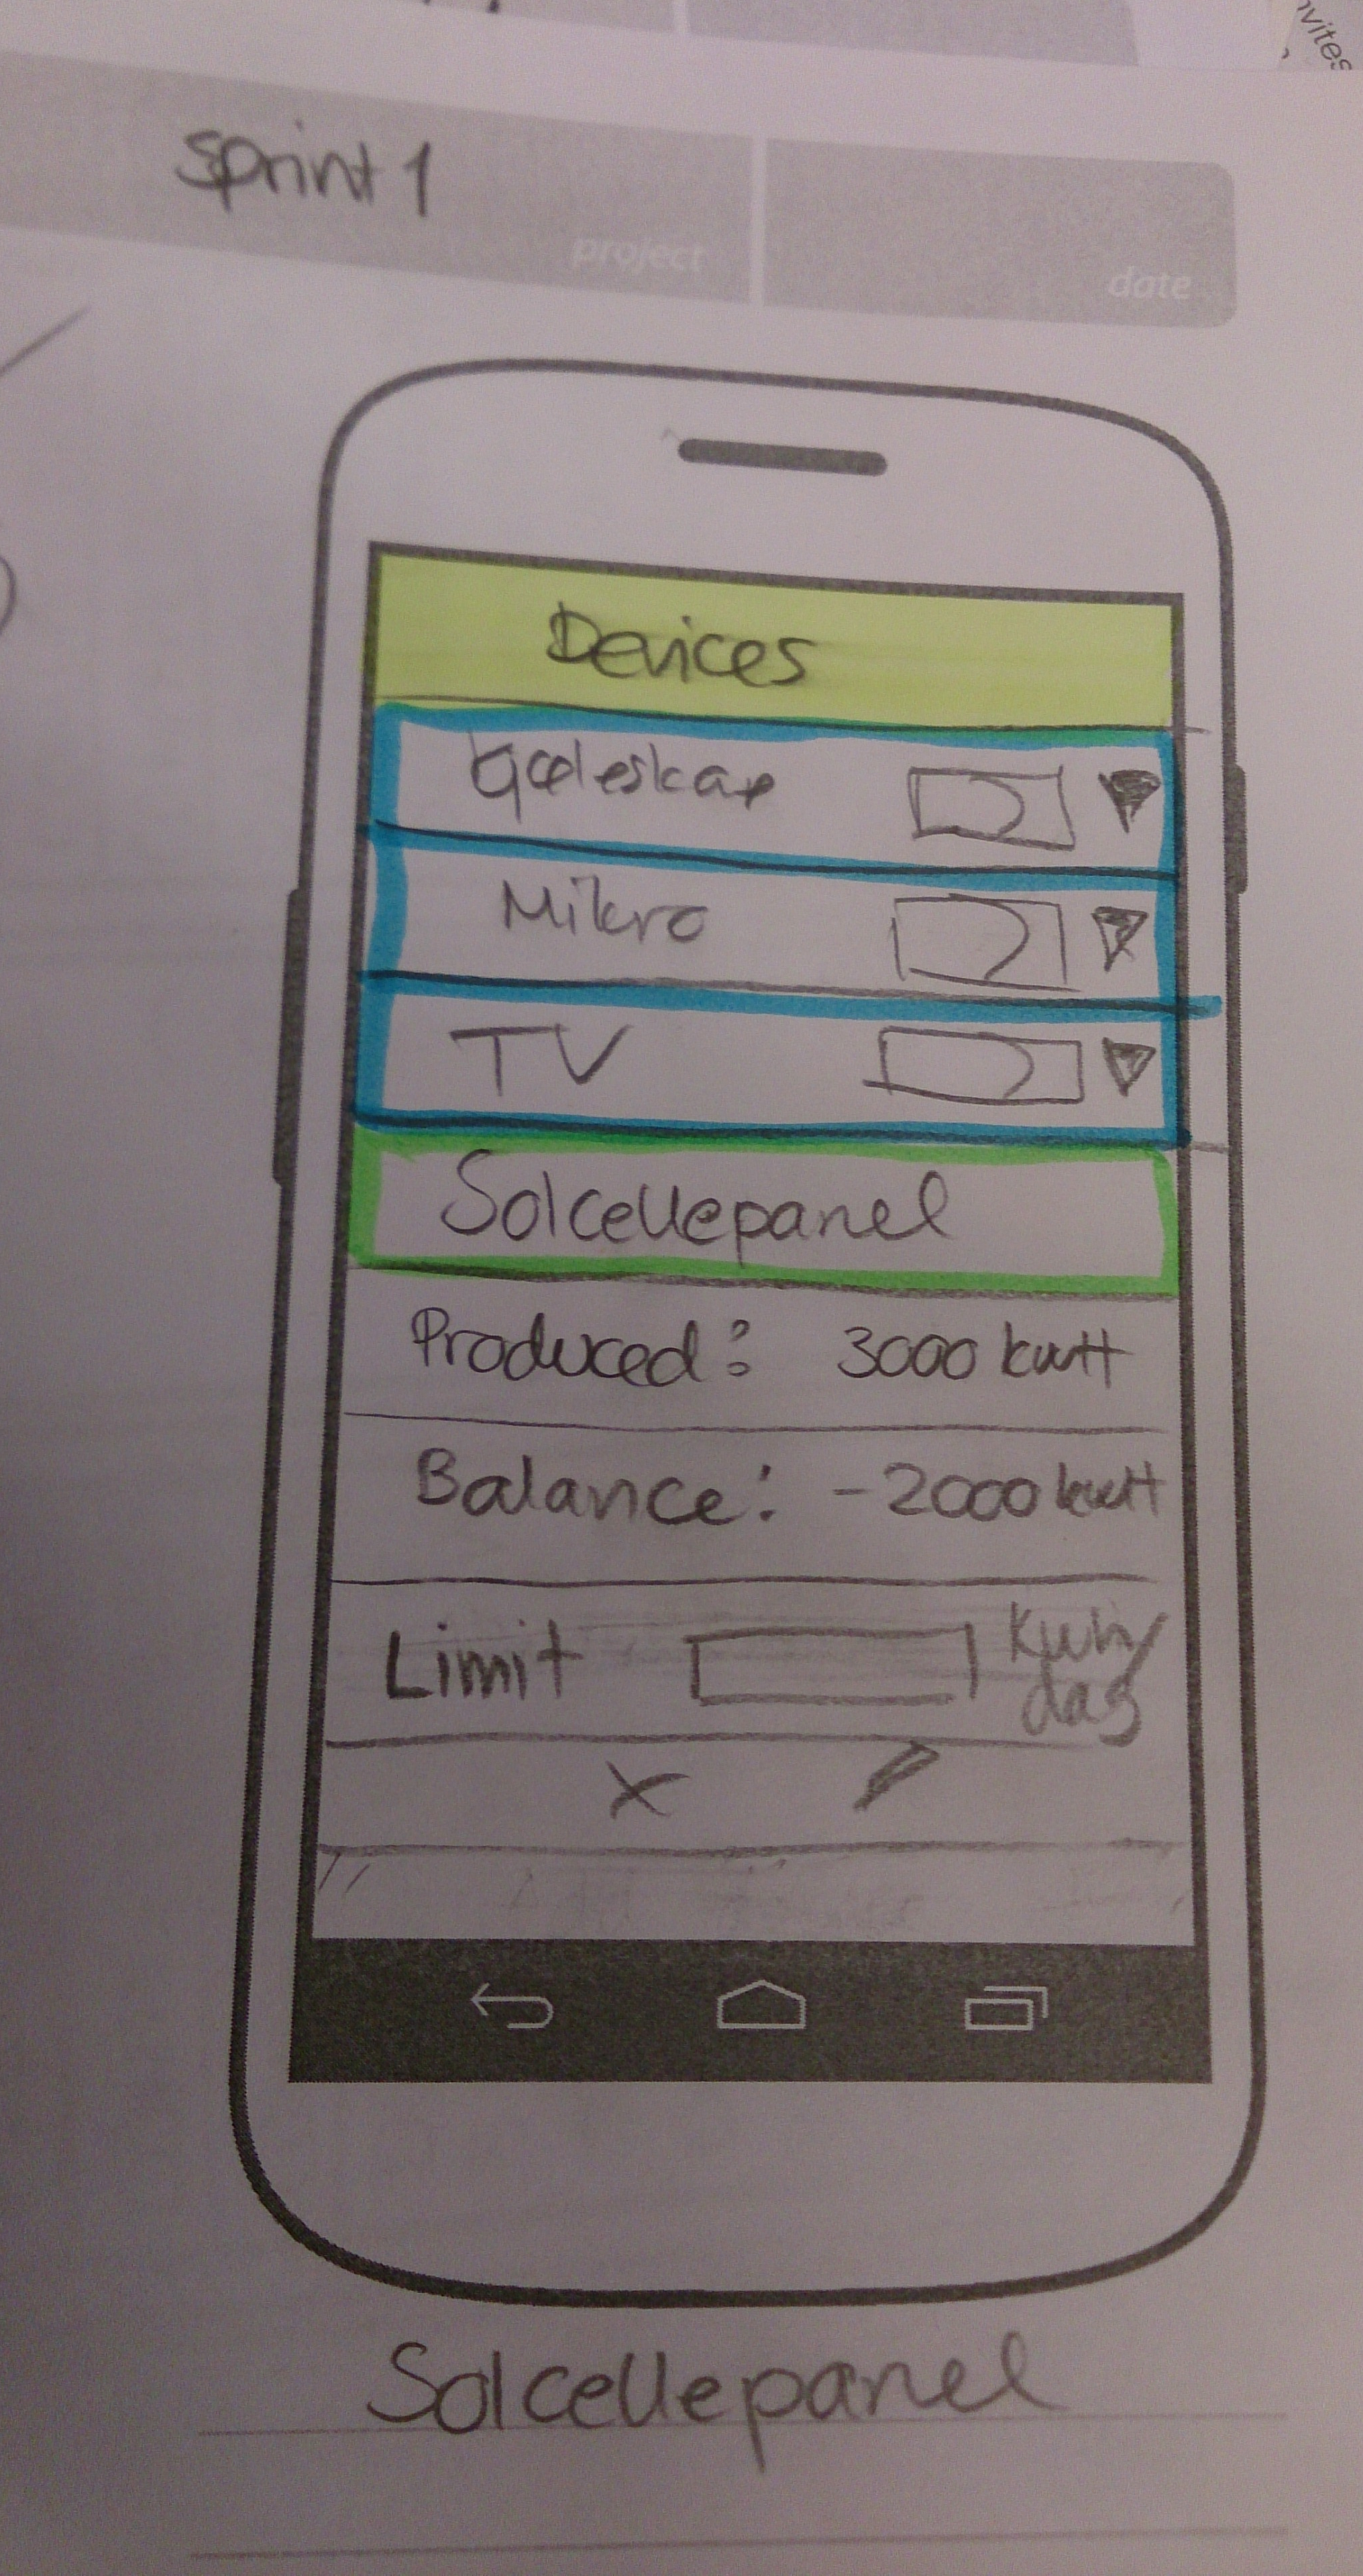
\includegraphics[width=0.3\textwidth, clip, trim= 6cm 4cm 2cm 16cm]{ch/devProcess/fig/paperprototype.png}}
\quad
  \subbottom[\label{fig:protob} Digitalized prototype of list of devices on proto.io]{%
\includegraphics[width=0.3\textwidth]{ch/devProcess/fig/device.png}}
\quad
  \subbottom[\label{fig:protoc} Screenshot of list of devices in app]{%
\includegraphics[width=0.3\textwidth, clip, trim= 0cm 4cm 19.8cm 0cm]{ch/devProcess/fig/app.png}}
\caption{The evolution: From prototype to product}
\end{figure}

\noindent However, a paper-prototype may have some drawbacks, as suggested by Snyder~\cite{paperprototype}. For instance, it is hard to incorporate changes without having to re-do work. It is static, and does not give the right impression on what the end product might look like. Therefore, the team moved on to a digital solution, namely the web page proto.io~\cite{protoio}. This tool made it possible to create dynamic prototypes. An example screenshot of this prototype is shown in figure~\ref{fig:protob}.

After the prototyping was done, the app was implemented in Android. An example screenshot of the finalized app is displayed in figure~\ref{fig:protoc}.
